\documentclass[10pt]{report}
\usepackage[pdftex]{graphicx}
\usepackage{hyperref}
\hypersetup{ colorlinks=true
           , linkcolor=cyan
           , pdfnewwindow=true 
           }
\usepackage{amsmath}
\usepackage{subfig}
\usepackage{listings}
\newcommand{\HRule}{\rule{\linewidth}{0.5mm}}
\hyphenation{auto-nomous}

% Limited by competition rules to min font size 10 pt, max pages 20

\begin{document}
\title{Rutgers Autonomous Aircraft Team\\Technical Report\\2010 AUVSI UAS Competition}
\author{Patrick Hickey et. al.}
\begin{titlepage}
\begin{center}

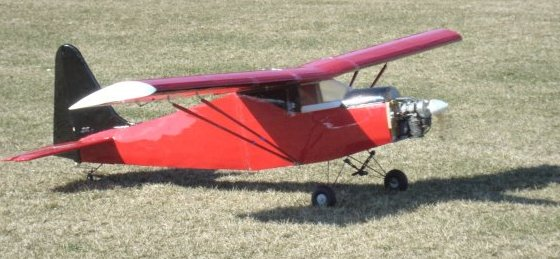
\includegraphics[width=0.5\textwidth]{../images/daedalus.jpg}\\[1cm]
\HRule \\[1cm]
{ \huge \bfseries Rutgers University Autonomous Aircraft Team } \\[0.5cm]
\HRule \\[0.5cm]
{ \large \bfseries Technical Report }
\\[0.5cm]
{ \large \bfseries 2010 AUVSI UAS Competition }
\\[0.5cm]
\HRule \\[1cm]

  {\large Amanda Gaetano, Anthony Garrison, Pat Hickey,}
\\{\large Stephen Indyk, Cogan Noll, John Palmer,}
\\{\large Adrien Perkins, Gregory Quinn, and Michael Varga}
\\[1cm]
\emph{Thank you to our sponsors}
\\ Rutgers University Engineering Governance Council
\\ Rutgers Alumni Association
\\ WINLAB
\\ Invensense, Inc.
\\ ST Micro, Inc.

\vfill
{\large \today}

\end{center}
\end{titlepage}


\begin{abstract}
we will put the abstract here.
\end{abstract}

\section{Introduction}

Brief overview of what we accomplished.

\section{Systems Engineering}

\section{Flight Vehicle}

\subsection{Airframe}

\subsection{Power}

\subsubsection{Engine}

\subsubsection{Batteries}

\section{Autopilot}
Our entry uses an autopilot system based off the open source 
Paparazzi project\cite{paparazziweb}. 
We ported the airborne code to Linux in order to use a single computer for all of our flight hardware and software.

\subsection{Requirments}

We needed to interface with the following hardware components:
\begin{itemize}
	\item GPS
	\item servos
	\item etc.
\end{itemize}

\subsection{Hardware}

\subsection{Software}

\subsection{Ground Station}

\subsection{Tuning and Testing}

\section{Imaging System}

\subsection{Camera}

\subsection{Image Processing}

\subsection{Ground Station Interface}

\section{Operation Safety}

\subsection{Safety Features}

\subsection{Procedures}

\bibliographystyle{plain}
\bibliography{paper}

\end{document}
